% Copyright (C) 2002-2006  Alexei Gilchrist and Paul Cochrane
% 
% This program is free software; you can redistribute it and/or
% modify it under the terms of the GNU General Public License
% as published by the Free Software Foundation; either version 2
% of the License, or (at your option) any later version.
%
% This program is distributed in the hope that it will be useful,
% but WITHOUT ANY WARRANTY; without even the implied warranty of
% MERCHANTABILITY or FITNESS FOR A PARTICULAR PURPOSE.  See the
% GNU General Public License for more details.
%
% You should have received a copy of the GNU General Public License
% along with this program; if not, write to the Free Software
% Foundation, Inc., 59 Temple Place - Suite 330, Boston, MA  02111-1307, USA.

% $Id: pyscriptElectronics.tex,v 1.7 2006/06/06 11:33:11 paultcochrane Exp $

\chapter{PyScript Electronics Object Package}

\section{Introduction}

This package is a library of standard symbols as used in electronic circuit
layout and design.  Thanks to Adrian Jonstone's lcircuit macros from CTAN
for the ideas and names.

\section{Objects}

\subsection{AND gate}
%%% AND gate
Draws a standard AND gate, with pins extending from the body of the gate.

Object options:
\begin{description}
\item[width:] The width of the object.
\item[height:] The height of the object.
\item[angle:] The rotation angle.
\item[pinLength:] The length of the pins extending from the gate.
\item[fg:] The foreground colour.  Use the \obj{Color} object to set this
option.
\item[bg:] The background colour.  Use the \obj{Color} object to set this
option.
\end{description}

\begin{figure}[h]
\centerline{\includegraphics[height=1cm]{electronics/AndGate}}
\caption{AndGate object}
\label{fig:and_gate}
\end{figure}

\subsection{NAND gate}
%%% NAND gate
Draws a standard NAND gate, with pins extending from the body of the gate.

Object options:
\begin{description}
\item[width:] The width of the object.
\item[height:] The height of the object.
\item[angle:] The rotation angle.
\item[pinLength:] The length of the pins extending from the gate.
\item[fg:] The foreground colour.  Use the \obj{Color} object to set this
option.
\item[bg:] The background colour.  Use the \obj{Color} object to set this
option.
\end{description}

\begin{figure}[h]
\centerline{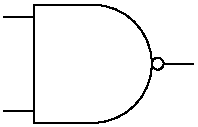
\includegraphics[height=1cm]{electronics/NandGate}}
\caption{NandGate object}
\label{fig:nand_gate}
\end{figure}

\subsection{OR gate}
%%% OR gate
Draws a standard OR gate, with pins extending from the body of the gate.

Object options:
\begin{description}
\item[width:] The width of the object.
\item[height:] The height of the object.
\item[angle:] The rotation angle.
\item[pinLength:] The length of the pins extending from the gate.
\item[fg:] The foreground colour.  Use the \obj{Color} object to set this
option.
\item[bg:] The background colour.  Use the \obj{Color} object to set this
option.
\end{description}

\begin{figure}[h]
\centerline{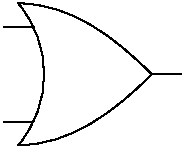
\includegraphics[height=1cm]{electronics/OrGate}}
\caption{OrGate object}
\label{fig:or_gate}
\end{figure}

\subsection{NOR gate}
%%% NOR gate
Draws a standard NOR gate, with pins extending from the body of the gate.

Object options:
\begin{description}
\item[width:] The width of the object.
\item[height:] The height of the object.
\item[angle:] The rotation angle.
\item[pinLength:] The length of the pins extending from the gate.
\item[fg:] The foreground colour.  Use the \obj{Color} object to set this
option.
\item[bg:] The background colour.  Use the \obj{Color} object to set this
option.
\end{description}

\begin{figure}[h]
\centerline{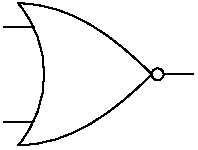
\includegraphics[height=1cm]{electronics/NorGate}}
\caption{NorGate object}
\label{fig:nor_gate}
\end{figure}

\subsection{XOR gate}
%%% XOR gate
Draws a standard XOR gate, with pins extending from the body of the gate.

Object options:
\begin{description}
\item[width:] The width of the object.
\item[height:] The height of the object.
\item[angle:] The rotation angle.
\item[pinLength:] The length of the pins extending from the gate.
\item[fg:] The foreground colour.  Use the \obj{Color} object to set this
option.
\item[bg:] The background colour.  Use the \obj{Color} object to set this
option.
\end{description}

\begin{figure}[h]
\centerline{\includegraphics[height=1cm]{electronics/XorGate}}
\caption{XorGate object}
\label{fig:Xor_gate}
\end{figure}

\subsection{NXOR gate}
%%% NXOR gate
Draws a standard NXOR gate, with pins extending from the body of the gate.

Object options:
\begin{description}
\item[width:] The width of the object.
\item[height:] The height of the object.
\item[angle:] The rotation angle.
\item[pinLength:] The length of the pins extending from the gate.
\item[fg:] The foreground colour.  Use the \obj{Color} object to set this
option.
\item[bg:] The background colour.  Use the \obj{Color} object to set this
option.
\end{description}

\begin{figure}[h]
\centerline{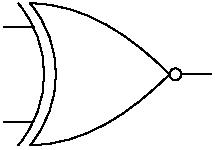
\includegraphics[height=1cm]{electronics/NxorGate}}
\caption{NxorGate object}
\label{fig:Nxor_gate}
\end{figure}

\subsection{NOT gate}
%%% NOT gate
Draws a standard NOT gate, with pins extending from the body of the gate.

Object options:
\begin{description}
\item[width:] The width of the object.
\item[height:] The height of the object.
\item[angle:] The rotation angle.
\item[pinLength:] The length of the pins extending from the gate.
\item[fg:] The foreground colour.  Use the \obj{Color} object to set this
option.
\item[bg:] The background colour.  Use the \obj{Color} object to set this
option.
\end{description}

\begin{figure}[h]
\centerline{\includegraphics[height=1cm]{electronics/NotGate}}
\caption{NotGate object}
\label{fig:not_gate}
\end{figure}

\subsection{Resistor}
%%% Resistor
Draws a standard resistor symbol, with pins extending from the body of the
symbol.

Object options:
\begin{description}
\item[width:] The width of the object.
\item[length:] The length of the object.
\item[angle:] The rotation angle.
\item[pinLength:] The length of the pins extending from the gate.
\item[fg:] The foreground colour.  Use the \obj{Color} object to set this
option.
\item[bg:] The background colour.  Use the \obj{Color} object to set this
option.
\end{description}

\begin{figure}[h]
\centerline{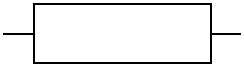
\includegraphics[height=1cm]{electronics/Resistor}}
\caption{Resistor object}
\label{fig:resistor}
\end{figure}

\subsection{Capacitor}
%%% Capacitor
Draws a standard capacitor symbol, with pins extending from the body of the
symbol.

Object options:
\begin{description}
\item[width:] The width of the object.
\item[sep:] The separation of the two plates of the capacitor.
\item[angle:] The rotation angle.
\item[pinLength:] The length of the pins extending from the gate.
\item[fg:] The foreground colour.  Use the \obj{Color} object to set this
option.
\item[bg:] The background colour.  Use the \obj{Color} object to set this
option.
\end{description}

\begin{figure}[h]
\centerline{\includegraphics[height=1cm]{electronics/Capacitor}}
\caption{Capacitor object}
\label{fig:capacitor}
\end{figure}

